\subsection{The facts, and just the facts}

It is not unusual to make the mistake of trying to give the user too much information, offering unnecessary or redundant data.
We don't want the user to be distracted or lost in the middle of a technically complete, but overly complex dataset. \\

The objective is not to create users with specialized knowledge of the field of your data, but rather to provide them with the
information in a way that they can apply to their daily life and thus improve it. Showing
technical, difficult to interpret data will only deter the user. \\

In complex cases, when dealing with concepts that are not in the users' comfort zone, we can use complementary, derived, or correlated data,
so that the user can be informed about the underlying reality that the data represents.
This practice can provide the user with a greater mastery of the concepts and they can be more
sure of their understanding. We can direct the user to other sources of information, where they can
get a more formal explanation if they wish, reinforcing the credibility of the representations we are making.
This should be entirely optional, and de-emphasised, because you typically can make no guarantees of external data characteristics.

\subsubsection*{Suggested strategies}

\begin{itemize}
    \item Focus on the objective - show only the data directly related to our goal
    \item Don't include the data simply because it appears in the dataset
    \item Don't include distracting technical details irrelevant to the user.
\end{itemize}

\subsubsection*{In the context of Aire Guru \ldots} 

The dataset used contains elements such as the identifier of the measurement station, whether the station is fixed or mobile
and extra data that is provided by the company that collects the data. This data is not useful for us.
For our website, only the coordinates of the measurement station have been used, as well as the time at which the measurement was recorded,
and the most relevant value of the five pollutants Co, No2, O3, Pm1, Pm 2.5 and Pm10.\\

In addition, while the measurement is unique for everyone, the general concept (the AQI) is common, and the ranges are the same for all users.
Thus the user has only a single concept to grasp. Exact measurements have been given - this data is quite technical for the user, but 
it lends veracity to the data. Therefore we have given it a secondary position to avoid distraction.\\

If the measure does not exist, we simply ignore it. We do not provide explanations or values such as 0 that can be mis-interpreted, erroneously reading as if there was no pollution.\\

In the following figure we see the difference between the zone and personal histories. The first of them does not show
the point where the measure was taken since it has been selected in the main map.\\

% TODO: not sure what this means
% We also like for the history of
% zone there is no filter for hours, since the measurements are reported every hour, this means that we will not find
% intermediate measures in the dataset.\\

\begin{figure}[ht]
    \centering
    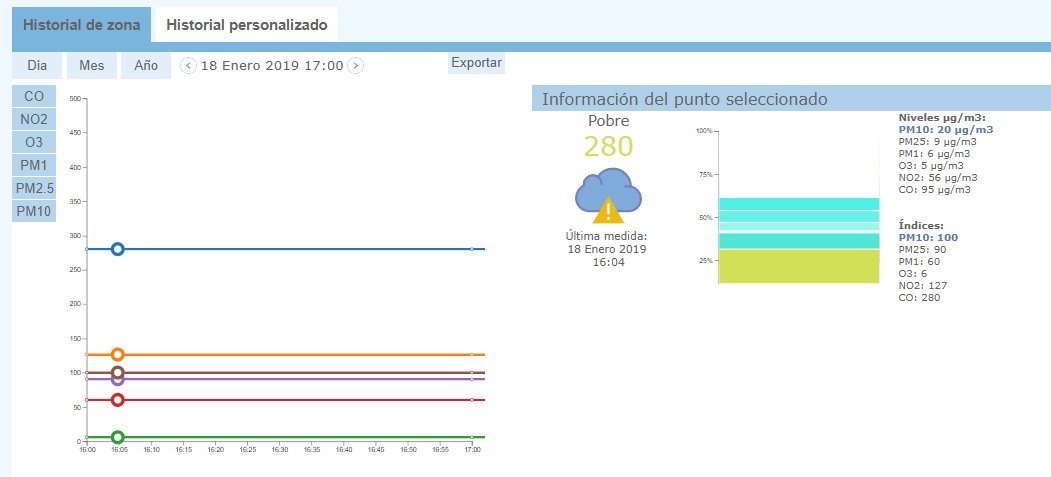
\includegraphics[width=11cm]{Figure_5_1_1_aireGuru_zoneRecords}
    \caption{ Zone Records}
\end{figure}
\begin{center}
    \bf{ 
    Figure 5.1.1. Zone Records}
\end{center}

\begin{figure}[ht]
    \centering
    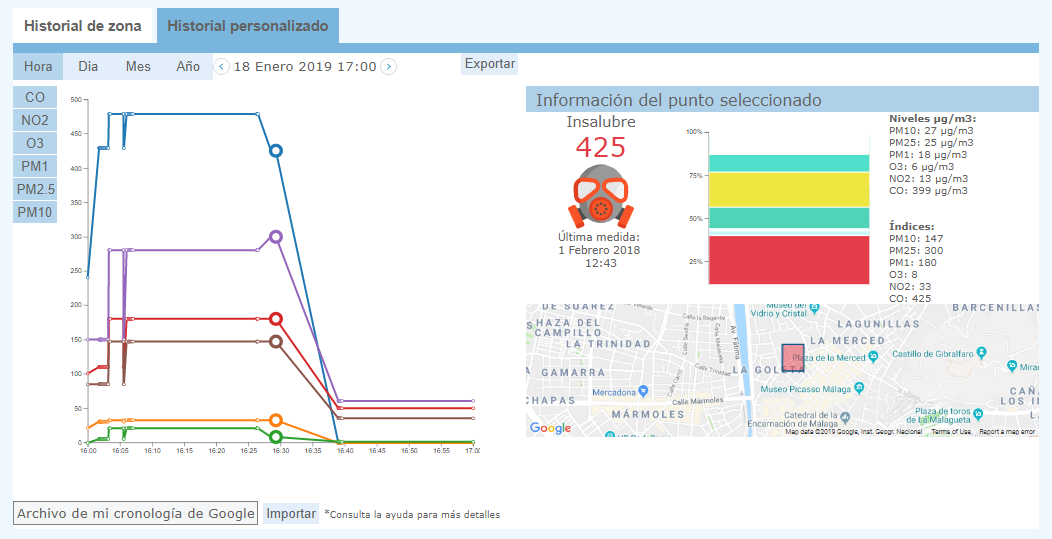
\includegraphics[width=11cm]{Figure_5_1_2_aireGuru_personalRecords}
    \caption{ Personal Records}
\end{figure}
\begin{center}
    \bf{ 
    Figure 5.1.2. Personal Records}
\end{center}

Aire Guru provides the user with the ability to export the data. The comments of our testers revealed
that this functionality is not useful for the average user, since they do not have the necessary tools to
analyse the data and all the information is represented in a better format in the website itself.